\documentclass[aps,prl,reprint,10pt,amsmath,amssymb,superscriptaddress,a4paper]{revtex4-2}

% Getting Helvetica Font
\renewcommand*\familydefault{\sfdefault}
\usepackage[scaled]{helvet}
\renewcommand\familydefault{\sfdefault} 
\usepackage[T1]{fontenc}

\usepackage{graphicx, float} % Graphics package
\usepackage{dcolumn, booktabs} % Double column package
\usepackage{amsmath,amsfonts,amsthm} % Math package

\usepackage[margin=2cm]{geometry} % Sets 2cm margins
\usepackage{datetime} % Package for automatic date & time

\usepackage{hyperref}

\setcitestyle{square}
\begin{document}
\title{CHEM2011: Carbon Monoxide Rotational Vibrational Spectrum Analysis}

\author{S.J. Shelton (z5359712)}
\affiliation{Friday AM class}
\affiliation{Word count: 1639 words}
\date{\currenttime~\today}

\begin{abstract}
A high-resolution infrared spectrum of gaseous Carbon Monoxide (CO), taken at room temperature and atmospheric pressure, is examined for characteristic rotational structure between 2000 and 2200 wavenumbers. The rotational structure is assigned, and both quadratic and cubic functions are used comparatively to extract rotational constants of interest. The cubic function is found to have a stronger correlation to experimental data than the quadratic (through a comparison of residuals), likely because the $x^3$ term accounts for centrifugal distortion. Gathered constants are used to determine the equilibrium rotational constant, $B_e$, as $1.9312(10)$, which is within experimental precision of the existing accepted value of $1.9313$ \cite{NIST}. The usefulness of Carbon Monoxide (and the determined values) to determine the temperature of astronomical bodies is discussed, and basic models using a Boltzmann distribution and experimental data are constructed.
\end{abstract}

\maketitle
% You start your main text after here.

\section{Introduction}

Carbon monoxide is a very useful compound for chemist and astronomers alike. As a diatomic molecule, its rotational structure is particularly well defined and easy to study, and unlike other common diatomic gasses like Nitrogen and Hydrogen gas ($\textnormal{H}_2$ and $\textnormal{N}_2$ respectively) it has a dipole meaning it is IR active. This allows carbon monoxide to be used as a reference point for various applications in cosmology, notably in the determination of the temperature of stellar objects like nebula.

This use case as a reference necessitates the precise analytical measurement of various properties of the molecule. These include, but are not limited to, the various rotational constants ($B_v$) and bond lengths ($r_v$), and by extension the equilibrium rotational constant and bond length ($B_e$ and $r_e$ respectively). It is through the precise measurement of these properties that we can effectively model the rotational structure of the IR spectrum as a function of temperature, and these models can be in turn applied to spectra gathered from interstellar bodies to predict their temperature.

\begin{equation}
\label{eqn:B}
B_e = \frac{h}{8 \pi^2 c \mu r_e^2}, \qquad \mu = \frac{m_1 m_2}{m_1 + m_2} 
\end{equation}

In this experiment, a research grade spectrometer is used to take a precise IR spectrum of gaseous carbon monoxide (CO) at room temperature and pressure; the rotational structure of note (between about 2000 and 22000 wavenumbers) is then assigned, with P and R branches being identified (reference figure \ref{fig:transitions}). A curve is then fitted to the data to extract $B_1$, $B_0$ and $\omega$, which are then in turn used to calculate $B_e$ and $r_e$. These values are compared to published literature to gauge experimental accuracy and precision.

This process is repeated for quadratic and cubic fits, and the two are quantitively and qualitatively compared. The data is then used to make a basic model based on a Boltzmann distribution that can be used to predict the temperature of stellar bodies. This model is ‘sanity checked’ by using it to calculate what the temperature of the sample the spectra was gathered from and comparing this to expectations of room temperature.

\begin{figure}[t]
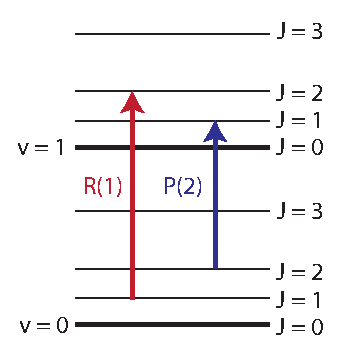
\includegraphics[width = 5 cm]{Transitions.eps}
\caption{Energy Transitions Diagram}
\label{fig:transitions}
\end{figure}

\section{Experimental Methods}

Data was recorded using a {SPECTROMETER NAME} FT IR spectrometer, using a high resolution and by averaging 64 scans to ensure usable, high-resolution data.

In order to correctly model the global precession of the data, both a cubic and a quadratic function were used and compared. These functions were defined as follows in \ref{eqn:fit}, with the quadratic version simply emitting the cubic term, i.e., $ D = 0$. Note that $D$ is just an arbitrary constant, whose physical meaning will be discussed later.

\begin{equation}
\label{eqn:fit}
\Delta S = \omega + \left( B_1 + B_0 \right) x + \left( B_1 - B_0 \right) x^2 + D x^4,
\end{equation}

\[ x = 
\begin{cases}
J + 1, \qquad J \in \textnormal{ R Branch }  \\
-J,    \qquad  \quad J \in \textnormal{ P Branch}
\end{cases}
\]

Data processing was done largely in \textsc{Python 3}, with \textsc{Mathematica} being used for some algebra and unit conversions. \textsc{SciPy} ( and several of its daughter packages), \textsc{NumPy} and \textsc{Matplotlib} were used extensively. Python code, raw data , {\LaTeX} files and illustrations can be found on \textsc{GitHub}\cite{GitHub}. Error handling was done natively within these packages.

\begin{figure*}[t]
\centering
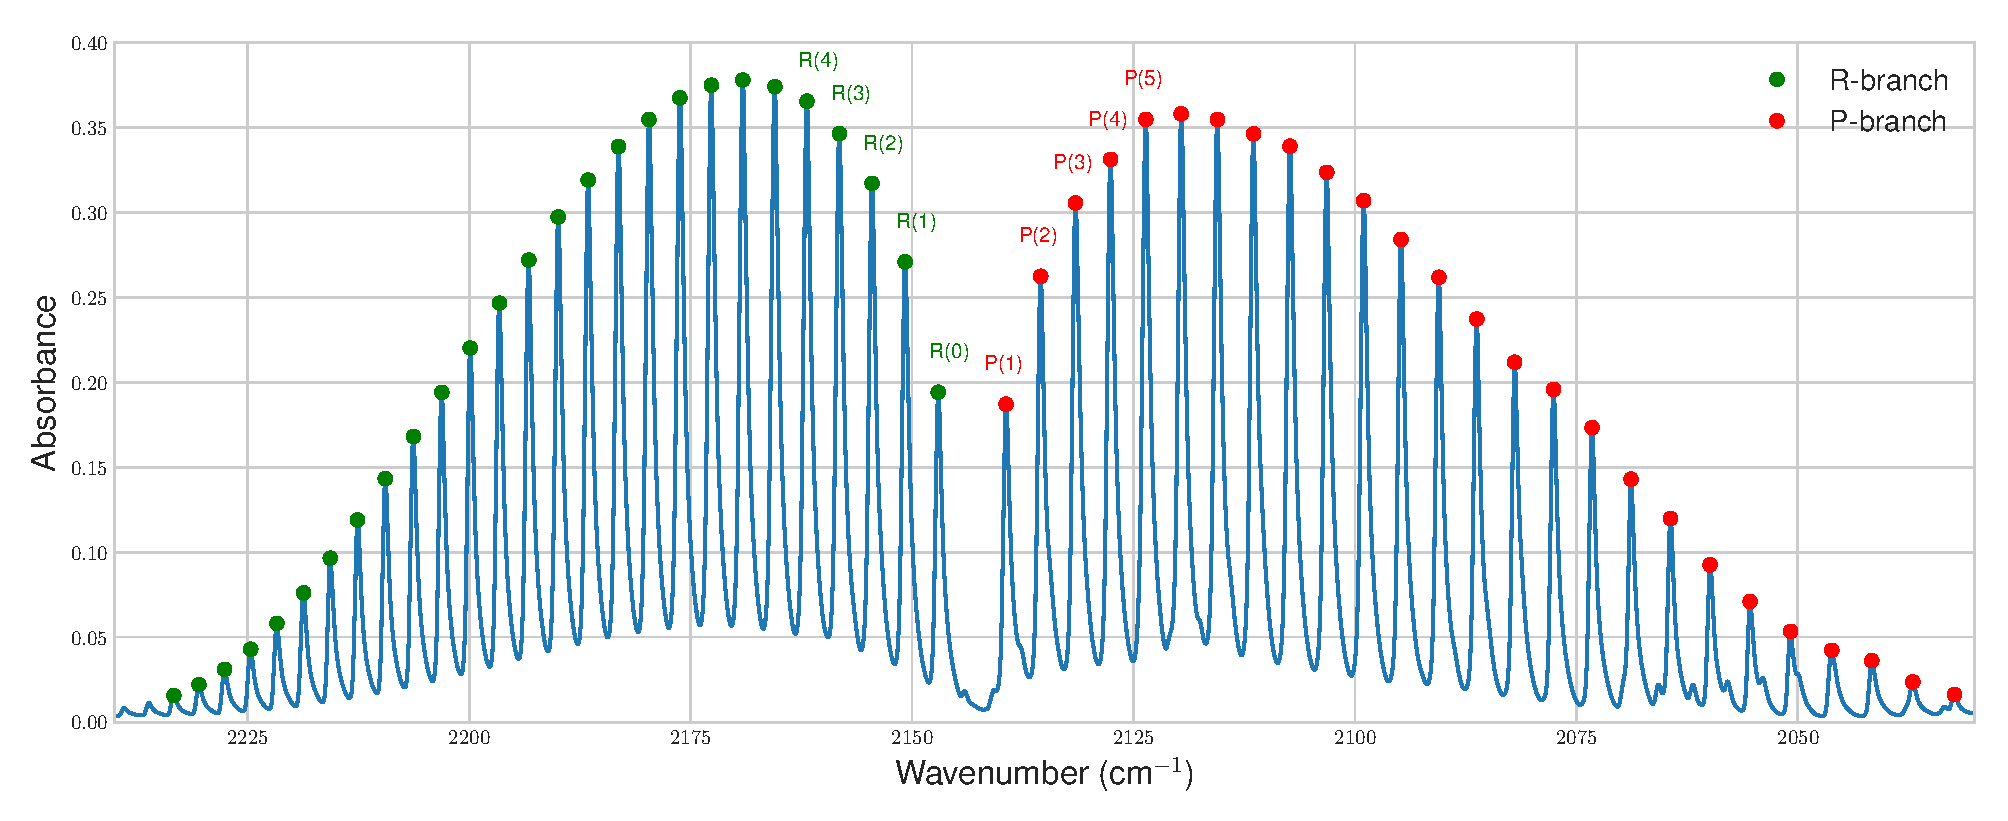
\includegraphics[width = 16 cm]{FormalExport.eps}
\caption{Fully assigned CO spectra, with some specific point labels omitted for clarity.}
\label{fig:spectra}
\end{figure*}

\section{Results}

Peaks were assigned as shown in figure \ref{fig:spectra}. The function in \ref{eqn:fit} was then fitted to extract $B_0$, $B_1$ and $\omega$ for both the quadratic and cubic case, with uncertainties from the fitting. These values were then used to calculate $B_e$ and $\alpha_e$ by solving $B_\nu = B_e - \alpha_e \left( \nu + 0.5 \right)$ for $\nu = 0$ and $1$ simultaneously, Then, equilibrium bond length was calculated using \ref{eqn:B}. More details can be found in the experimental notes\cite{notes}. The results are shown in table \ref{tab:results}, and the cubic fit is shown graphically in figure \ref{fig:Cubic}.

\begin{figure}[H]
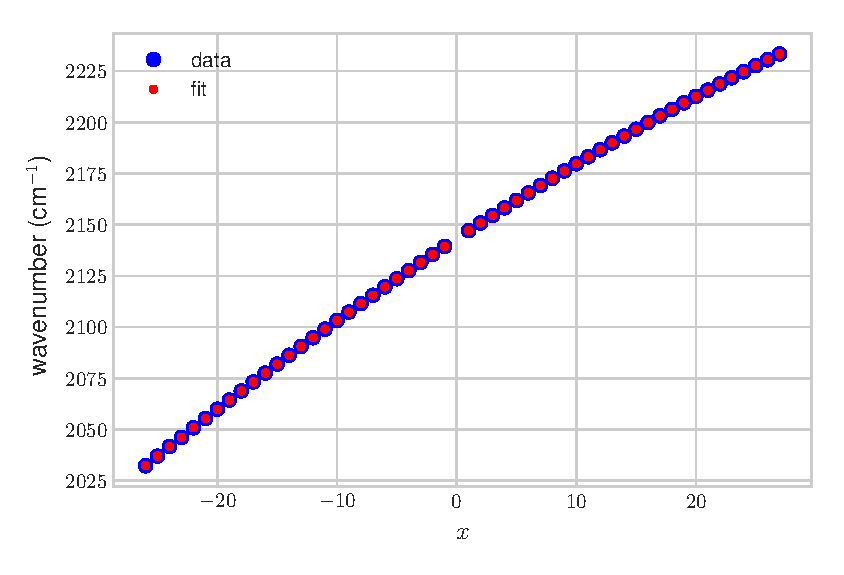
\includegraphics[width = 8 cm]{CubeFit.eps}
\caption{Cubic fit of Global Progression}
\label{fig:Cubic}
\end{figure}

\begin{table}[h]
\begin{tabular}{@{}lllllll@{}}
\toprule
                         & Cubic Fit    		& Quadratic Fit 		& Literature	&Units		& \\ \midrule
$B_0$          	& $1.9224(10)$       	& $1.8998(14)$         &$1.9225$ 	&cm$^{-1}$	& \\ 
$B_1$   		& $1.9054 (10)$      	& $1.9172(14)$         &$1.9051$	&cm$^{-1}$	& \\ 
$B_e$    		& $1.9312(10)$       	& $1.9260(14)$         &$1.9313$ 	&cm$^{-1}$	& \\
$\alpha_e$    	& $0.0174(15)$       	& $0.0175(19)$         &$0.0175$ 	&cm$^{-1}$	& \\ 
$\omega$ 	& $2143.190(13)$  	& $2143.192(32)$ 	&$2169.814$ 	&cm$^{-1}$	& \\ 
$r_e$   		& $1.1282(15)$       	& $1.1295(80)$         &$1.1283$	&\AA			& \\ \bottomrule
\end{tabular}
\caption{Experimental Constants Comparison \cite{NIST}\cite{MolSpectra}\cite{Education}}
\label{tab:results}
\end{table}

\pagebreak

To further investigate the two models, it is rescissory to compare their accuracies by calculating their respective sum of residuals. We find that the cubic and quadratic fits have a residual sum of squares of $0.0291$ and $0.3025$ respectively, within the context of absorbance values within about $0.05$ and $0.35$. This is favourable to the cubic model, and this trend continues when we plot the residuals as in figure \ref{fig:Residuals}.

\begin{figure}[h]
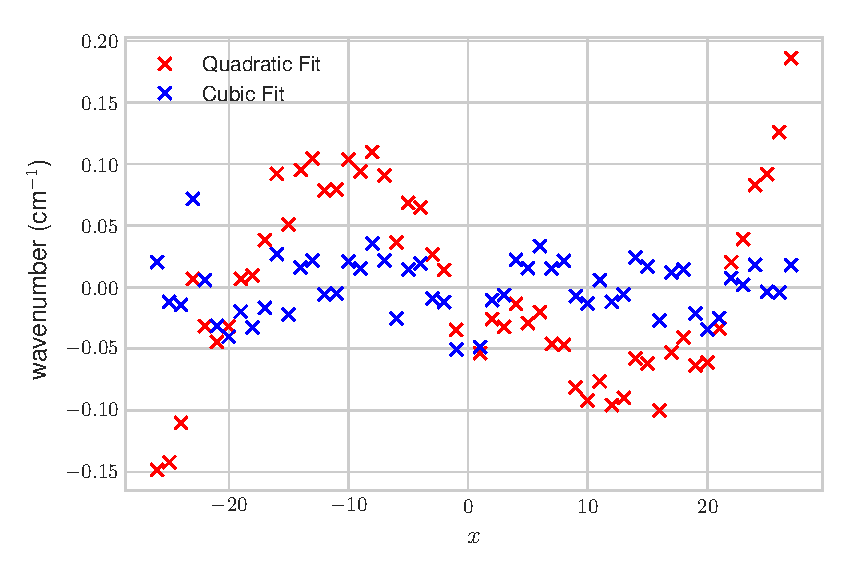
\includegraphics[width = 8 cm]{Residuals.eps}
\caption{Plot of Residuals}
\label{fig:Residuals}
\end{figure}

It should be clear that the residuals of the quadratic plot have a clear cubic pattern; this result suggests that adding a cubic term would be much more appropriate for this data. This conclusion concurs with the conclusions from both the residual comparison and with the relative accuracy of the cubic model with regards to data from literature.

Finally, it is useful to attempt to fit a Boltzmann distribution to the intensity of the R branch to extract thermal data. Fitting equation \ref{eqn:Boltz} to the R branch data exclusively yields the following plot (figure \ref{fig:Thermals}) and a thermal value of $289$ K, or $15.9$ C. This graph will be scrutinised more in the discussion, but for now just note that the fit is far from excellent.

{\it n.b.} in \ref{eqn:Boltz}, $\lambda$ is just some constant of proportionality.

\begin{equation}
I \left( J \right) = \lambda \times \left( 2J + 1 \right) e^{ - B_0 J \left( J + 1 \right) /k_B T}
\label{eqn:Boltz}
\end{equation}

\begin{figure} [h]
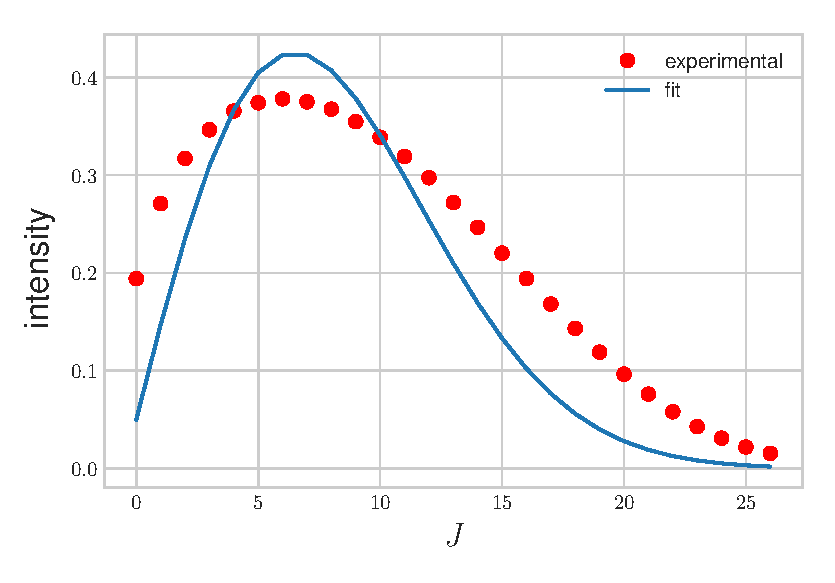
\includegraphics[width = 8 cm]{Thermal.eps}
\caption{Fitted Boltzmann Distribution to R Branch}
\label{fig:Thermals}
\end{figure}

\section{Discussion}

Clearly the cubic term was the correct fit, but it is important to understand why. There are two key approximations that we have made in order to construct our model of diatomic rotational spectroscopy. These are the quantum harmonic anharmonic oscillator and the quantum rigid rotor. 

More specifically, instead of using the quantum anharmonic oscillator we used a morse potential: an approximation of the infinite anharmonic series to a simple quadratic. This would explain why adding in higher order turns increases the accuracy of the fit, although it is important to note that adding too many higher order terms could become problematic; a polynomial of sufficient degree will perfectly fit any set of data, and coefficients will eventually lose any physical meaning.

The second approximation is the quantum rigid rotor. This is itself a contradiction with the first assumption. The diatomic bond cannot be both spring-like (an oscillator) and a rigid rotor. A non-rigid rotor has additional, higher order terms to account for centrifugal distortion and other effects. At higher rotational quantum numbers, it makes intuitive sense that the bond should get longer (and hence $B$ should get smaller). A cubic centrifugal distortion term helps account for this.

Together, these two points help to explain, in physical terms, why adding a cubic term improves the goodness of fit, beyond any improvement that would emerge simply from using a higher order polynomial.

Additionally, we should consider why the Boltzmann-derived thermal fit, shown in fire \ref{fig:Thermals}, is so poor. The explanation is straightforward; the spectra was recording at room temperature and pressure. While the curve fit extracts an appropriate temperature ($15$ C seems very reasonable, it was a very cold day) the fit itself is not very satisfying. 

Recording the temperature at atmospheric pressure distorts the relative absorbance peaks. As Van Krefeld and Van Der Elksen note\cite{Pressure}, we should expect to see a greater difference in the intensity of adjacent rotational transitions at higher temperatures. This explains the deviation from the expected distribution.

An additional source of some of this error might be the saturation of the experimental apparatus. Sample data (provided in the QS4 analysis lab) has absorbance peaks roughly an order of magnitude less than gathered experimental data. In his paper investigating the effects of saturation in FTIR spectroscopy, Grdadolnik shows how increasing concentrations of the compounds of interest can conceal the true magnitude and detail of FTIR absorbance peaks\cite{Saturation}. This effect could certainly have contributed to the observed data.

Note that the thermal results are dependent on the relative {\it intensity} of rotational peaks, while the rotational results are dependent on their relevant {\it energies}. This means that we can get great results for the rotational constants while having not very useful thermal data.

\section{Conclusions}

An infrared rotational spectra of CO was assigned and analysed, with rotational constants extracted. A cubic model was determined (by analysis of residuals) to be the most appropriate, and the value of $B_e$ was determined experimentally to be $1.9312(10)$ cm$^{-1}$, within experimental precision of the existing accepted value of $1.9313$ cm$^{-1}$ \cite{NIST}. This trend continued for other rotational constants. 

Physical justifications for the cubic model's superiority were explored, and a Boltzmann relationship was plotted against peak intensity to determine thermal properties. Inaccuracies in these models were discussed.

\begin{thebibliography}{99}

\bibitem[]{NIST} National Institute of Standards and Technology (NIST), U.S. Department of Commerce, 2021, {\it Carbon Monoxide}, NIST Chemistry WebBook, SRD 69, \href{https://webbook.nist.gov/cgi/cbook.cgi?ID=C630080}{accessed July 2022}. 

\bibitem[]{GitHub} A GitHub repo containing code used can be found \href{https://github.com/Sam-js2/CHEM2011-Lab-Report}{here}.

\bibitem[]{notes} Experimental Notes were provided on moodle, there is also a copy in the repo\cite{GitHub}.

\bibitem[]{MolSpectra} Rank, D, St Pierre, A \& Wiggins, T 1965, ‘Rotational and Vibrational Constants of CO’, {\it Journal of Molecular Spectroscopy}, vol. 18, no. 4, \href{https://www.sciencedirect.com/science/article/abs/pii/0022285265900482}{pp. 418-427}.

\bibitem[]{Education} Mina-Camilde, N, Manzanares, C \& Caballero, J 1996, ‘Molecular Constants of Carbon Monoxide at v = 0, 1, 2, and 3: A Vibrational Spectroscopy Experiment in Physical Chemistry’, {\it Journal of Chemical Education}, vol. 73, no. 8, \href{https://doi.org/10.1021/ed073p804}{pp. 695-826}. 

\bibitem[]{Pressure} Van Krefeld, ME \& Van Der Elsken, J 1968, ‘A comparison of the pressure effect on the pure rotational and vibration rotation spectra of HCl’, {\it Chemical Physics Letters }, vol. 1, no. 11, \href{ https://www.sciencedirect.com/science/article/pii/0009261468800119}{pp. 532-534}.

\bibitem[]{Saturation} Grdadolnik, J 2003, ‘Saturation effects in FTIR spectroscopy: Intensity of Amide I and Amide II bands in protein spectra’, {\it Acta Chimica Slovenica}, vol. 50, \href{ https://www.researchgate.net/publication/228541251_Saturation_effects_in_FTIR_spectroscopy_Intensity_of_Amide_I_and_Amide_II_bands_in_protein_spectra }{pp. 777-788}.

\bibitem[]{textbook} T. Engel, 2019, {\it Quantum Chemistry and Spectroscopy}, 4th edn, Pearson Education, Inc, New York, USA.

\end{thebibliography}

\end{document}